\section*{Motivation}
Efficient team schedule planning is a complex challenge, particularly in organizations that require real-time coordination and resource management.
Existing scheduling services often have significant limitations, such as proprietary nature, lack of customization, and dependence on third-party infrastructure.
This highlights the need for tailored solutions that can address specific organizational requirements more effectively.
This project aims to develop a self-hosted open-source booking system designed for organizations that need a private, adaptable scheduling solution.
The system will provide a web-based interface where users can:
\begin{itemize}
    \item Make and manage reservations
    \item Check real-time room availability
    \item  Filter bookings by person or room
    \item View all reservations on a centralized calendar
\end{itemize}

The backend will be built using the Spring Framework, ensuring scalability, security, and ease of integration with existing infrastructure.
Unlike cloud-based alternatives, this system will store all data locally, giving organizations complete privacy and control over scheduling information.
By combining flexibility, transparency, and data privacy, this project can provide a practical alternative to commercial scheduling tools, empowering organizations with greater autonomy and customization options.
\addcontentsline{toc}{section}{Motivation}


\pagestyle{headings}
Here we will talk about why the calendar is needed

Firstly, let's take a look at the current solution used by my university, CTU. Rozvrh.fjfi.cvut.cz is a website where students can see their schedule.


\section{The current solution}\label{sec:the-current-solution}
\begin{figure}[h]
    \centering
    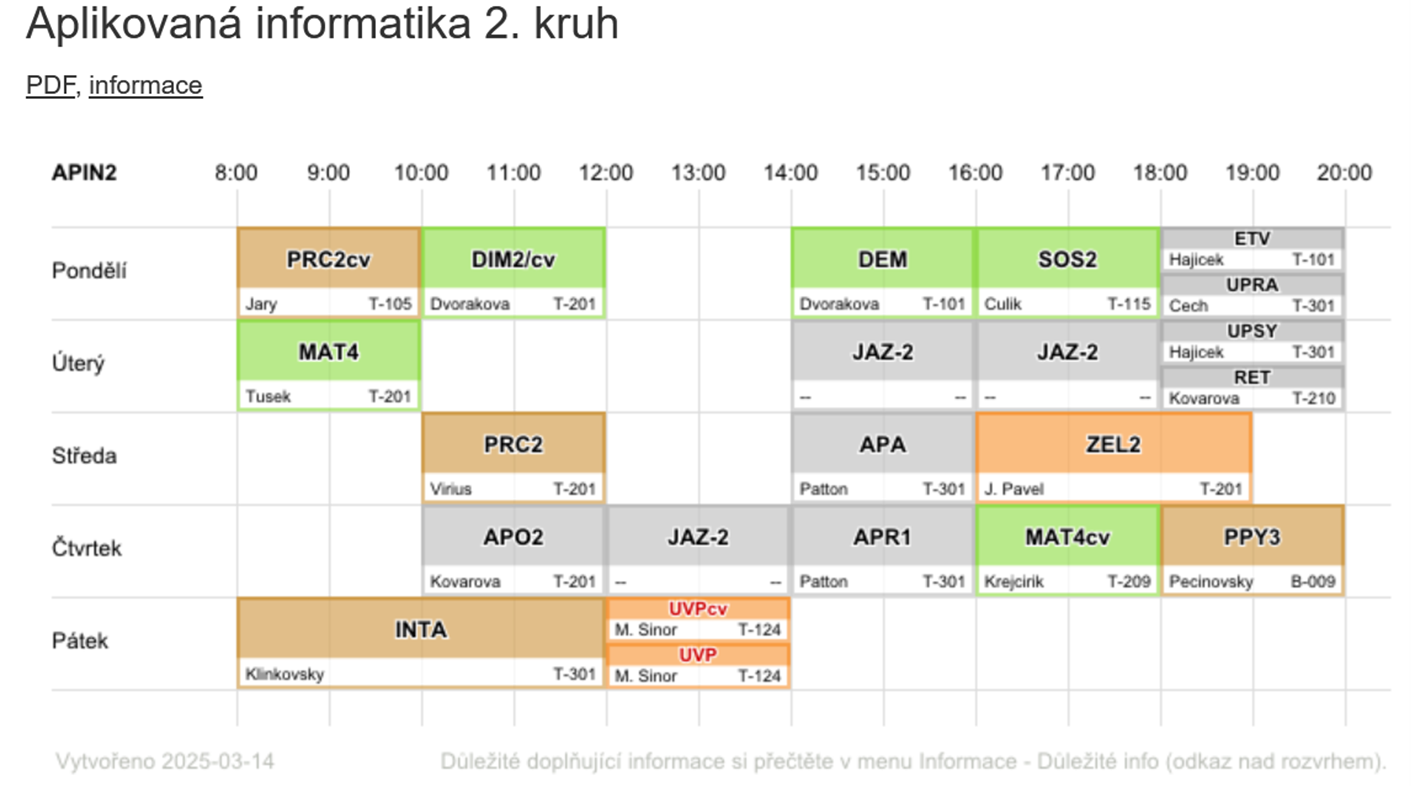
\includegraphics[width=0.6\textwidth]{img}
    \caption{Screenshot of the current solution}
    \label{fig:rozvrh}
\end{figure}

It can be seen on~\ref{fig:rozvrh} that while the website completes its main purpose, it is not customizable, which makes it hard to use.
For example, if a student has a class that is from another year or/and program, they have to look at another picture and manually compare them.
From my experience, many students have screenshots on their phones and they cross-out the classes that they are not registered to.
They may have a few screenshots, for different programs or years.
It is not a good solution, as it allows for misunderstandings and mistakes.

This is why a project focused on creating a calendar that is easy to use and customizable is needed.


\section{Theory}\label{sec:theory}

\subsection{Spring Boot}\label{subsec:spring-boot}
Spring Boot is a framework that simplifies the development of Java applications by providing a set of pre-configured templates and libraries.
It allows developers to easily create enterprise-level applications with minimal configuration.
Spring Boot is built on top of the Spring Framework, which is a popular framework for building Java applications.
Spring Boot provides a number of features that make it easy to develop and deploy applications, including:
\begin{itemize}
    \item Embedded web server: Spring Boot includes an embedded web server, which allows developers to quickly create and deploy web applications without the need for an external server.
    \item Auto-configuration: Spring Boot automatically configures the application based on the dependencies that are included in the project.
    \item Starter dependencies: Spring Boot provides a number of starter dependencies that make it easy to add common functionality to the application.
    \item Actuator: Spring Boot includes an actuator module that provides production-ready features such as health checks and metrics.
\end{itemize}


Although Spring Boot is a powerful framework, it can be complex and difficult to learn at first.
This was one of the problems that were encountered during the development of the project.
Navigating the documentation and understanding how to use the various features of Spring Boot took some time.
Especially given that Spring Boot is changing rapidly and the resources are showing what was in the past.
Many times the documentation encountered was outdated and did not work with the current version of Spring Boot.

This is why the next section will be dedicated to the explanation of the Spring Boot framework.

\subsection{Configuration of the Spring Boot project}\label{subsec:configuration-of-the-spring-boot-project}

\subsubsection{Security}
Spring Security is a powerful and customizable authentication and access control framework.
It is the standard for securing Spring-based applications.
Spring Security provides almost ready-to-use authentication and authorization features, which can be easily integrated into any Spring application.

In this project, Spring Security is configured to provide a robust security solution with the following components:

\begin{itemize}
    \item \textbf{JWT-based Authentication}: JSON Web Tokens (JWT) are used for stateless authentication.
    When a user logs in, a JWT token is generated and stored in a secure HTTP-only cookie.
    This token is then validated on each request.

    \item \textbf{Password Encoding}: BCryptPasswordEncoder is used to securely hash passwords before storing them in the database, ensuring that even if the database is compromised, the actual passwords remain protected.

    \item \textbf{CSRF Protection}: Cross-Site Request Forgery protection is implemented using a cookie-based CSRF token repository, with specific endpoints (like authentication endpoints) being exempted.

    \item \textbf{CORS Configuration}: Cross-Origin Resource Sharing is configured to allow requests only from trusted origins, enhancing security against cross-site attacks.

    \item \textbf{Stateless Session Management}: The application uses stateless session management, which means no session data is stored on the server,removing the need for session management and reducing server load.
    This also makes the application more scalable and secure.

    \item \textbf{Role-based Authorization}: Different endpoints are protected based on user roles.
    For example, API endpoints require the USER role, while configuration endpoints require the CONFIG role.
    User roles are stored in the database and associated with user accounts, allowing for flexible permission management.

    \item \textbf{Custom Token Filter}: A custom filter (TokenFilter) is implemented to extract and validate JWT tokens from either the Authorization header or cookies, setting up authentication for each request.
\end{itemize}

The security configuration is implemented across several classes:

\begin{itemize}
    \item \textbf{SecurityConfigurator}: Sets up the security filter chain, defines authorization rules, and configures various security features.

    \item \textbf{SecurityController}: Provides REST endpoints for user authentication (signin, signup, signout) and handles JWT token generation.

    \item \textbf{TokenFilter}: Validates JWT tokens and sets up authentication for each request, with special handling for public paths and different types of requests.

    \item \textbf{JwtCore}: Manages JWT token generation and validation, including setting token expiration, signing with a secret key, and extracting user information from tokens.
\end{itemize}

This security setup ensures that the application is protected against common web vulnerabilities while providing a seamless user experience.


\subsection{Storing the data}\label{subsec:storing-the-data}
In this project Spring Data JPA is used to store the data.
Spring Data JPA is a part of the Spring Framework that simplifies data access and manipulation in Java applications.
It allows developers to interact with databases using Java objects, eliminating the need for complex SQL queries and boilerplate code.
Elements of Spring Data JPA include:
\begin{itemize}
    \item \textbf{Repositories}: Spring Data JPA provides a repository abstraction that allows developers to define data access methods using interfaces.
    These repositories automatically implement common CRUD operations, reducing the need for boilerplate code.

    \item \textbf{Entities}: Entities are Java classes that represent database tables.
    Spring Data JPA uses annotations to map these classes to database tables, making it easy to perform operations on the underlying data.

    \item \textbf{Query Methods}: Developers can define custom query methods in repository interfaces using method names.
    Spring Data JPA generates the necessary SQL queries based on these method names, simplifying data retrieval.
    If the method name is not enough, the @Query annotation can be used to define custom queries.

    \item \textbf{Auditing}: Spring Data JPA provides built-in support for auditing entities, enabling automatic tracking of creation and modification timestamps.
\end{itemize}

\subsubsection{Useful tools}\label{subsubsec:useful-tools}
In this application, \textit{Lombok} was used to reduce the amount of boilerplate code.
It allows for the usage of annotations such as \texttt{@Getter,@Setter} to automatically generate setters and setters for all fields that need them.
In addition, annotations \texttt{@AllArgsConstructor,@NoArgsConstructor} can automatically create the correct construction function for the class.
Finally, \texttt{@Data} combines \texttt{@Getter,@Setter} and some more functions in one annotation, so the classes remain clean and functional.

The use of the tool is demonstrated in the list~\ref{lst:room-class}.
It can be seen that no setter or getter functions are needed, no construction function is needed, and the class looks clean and complete.


\begin{listing}[H]
    \begin{minted}{java}

@Data
@Entity
@Table(name = "rooms")
@EqualsAndHashCode(callSuper = true)
public class Room extends Auditable {
    @Id
    @GeneratedValue(strategy = GenerationType.IDENTITY)
    private Long id;

    @Column(nullable = false, unique = true)
    private String name;

    @Column()
    private String description;

    @Type(io.hypersistence.utils.hibernate.type.array.ListArrayType.class)
    @Column(name = "tags", columnDefinition = "text[]")
    private Set<String> tags = new HashSet<>();

}
    \end{minted}
    \caption{Lombok-annotated JPA entity}
    \label{lst:room-class}
\end{listing}


\subsection{Controllers and services}\label{subsec:controllers-and-services}
The application is divided into several parts, each responsible for a specific aspect of the application.
\begin{itemize}
    \item \textbf{Controllers}: Controllers are responsible for handling incoming requests and returning responses.
    They act as the bridge between the client and the service layer, processing user input and returning the appropriate data.

    \item \textbf{Services}: Services contain the business logic of the application.
    They interact with the repository layer to perform CRUD operations and implement any necessary business rules.

    \item \textbf{Repositories}: Repositories are responsible for data access and manipulation.
    They provide methods for querying and updating the database, abstracting away the underlying data access technology.
\end{itemize}

The controllers in this applications are divided into several parts:
\begin{itemize}
    \item \textbf{ConfigurationController}:This controller is separated into two parts.
    RestConfigController is responsible for handling the requests and returning the data, while ConfigController is responsible for displaying the pages.

    \item \textbf{Calendar Controller}: This controller is responsible for essential handling of calendar-related requests, such as retrieving available time slots, managing bookings and displaying calendar events.

    \item \textbf{Authentication Controller}: This controller manages user-related operations, including user registration, authentication, and profile management.

    \item \textbf{Error Controller}: This controller handles errors that may happen.
    It displays the error page and logs the error.
\end{itemize}

There are also several services that are responsible for the business logic of the application.
These are: \texttt{CalendarService}, \texttt{User Service}, and \texttt{Default Value Service}.


\texttt{CalendarService} is responsible for handling the calendar-related operations, such as retrieving available time slots, managing bookings, and displaying calendar events.
It is arguably the most important service in the application.


\texttt{DefaultValueService} is responsible for setting the testing values for the application.
It allows for easy stress-testing of the application and checking the stability of the application.

\texttt{UserService} is responsible for integrating user authentication into the Spring Security framework.
It implements Spring Security's UserDetailsService interface, which serves as the bridge between custom user database and Spring Security's authentication system.


\section{The solution}\label{sec:the-solution}
\begin{figure}[h]
    \centering
    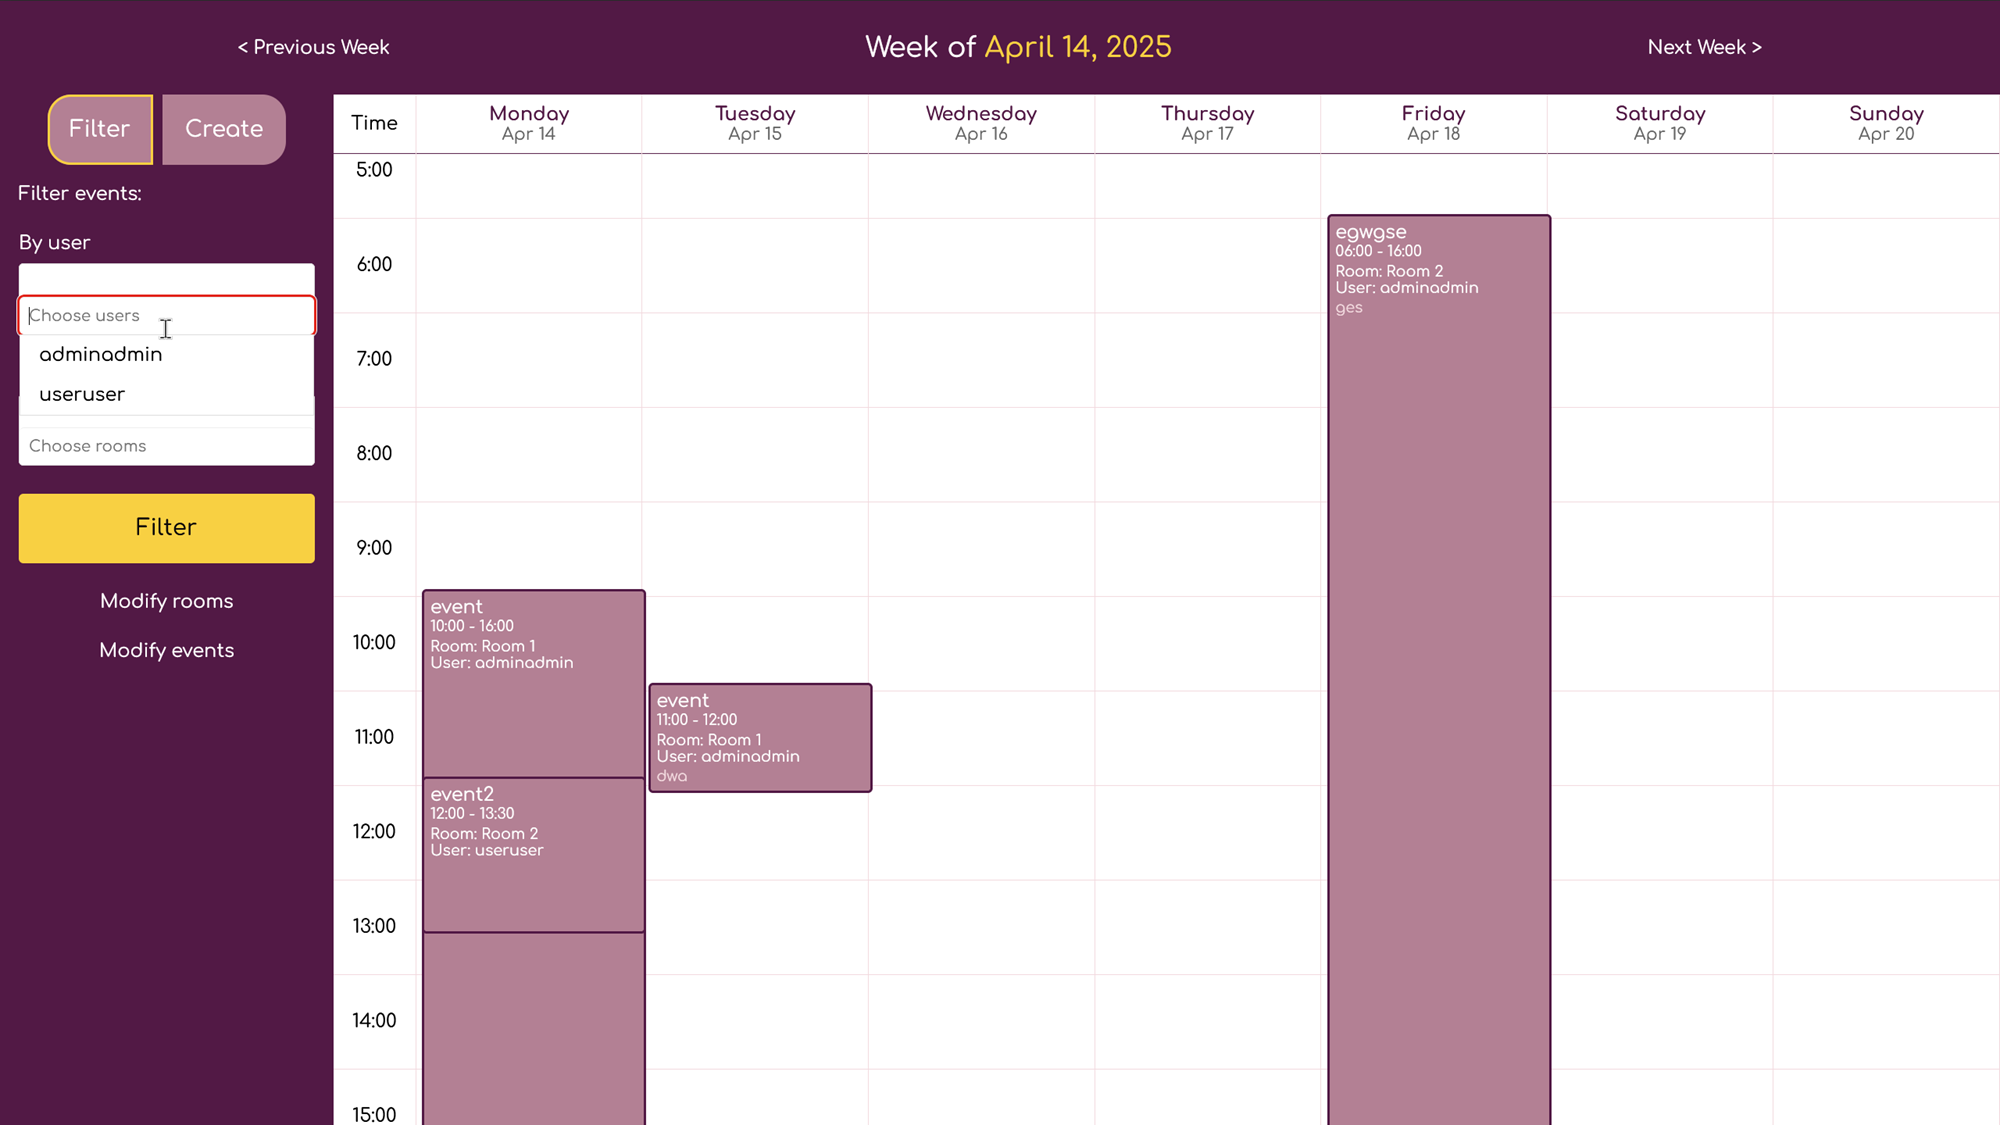
\includegraphics[width=0.6\textwidth]{TeamJob}
    \caption{Screenshot of the new solution}
    \label{fig:TeamJob}
\end{figure}
TeamJob is a web application that allows users to filter exactly what they want to see.
By default, all the events that are happening this week are shown.
The user can filter the events by the room and the person that is assigned to this event.
This allows for a more precise view of the calendar, where the user can see only the events that are important to them.
The user can also move between weeks.
A specific day-view allows the user to see the events that are happening on a specific day, if there are too many events to show them all at once.
